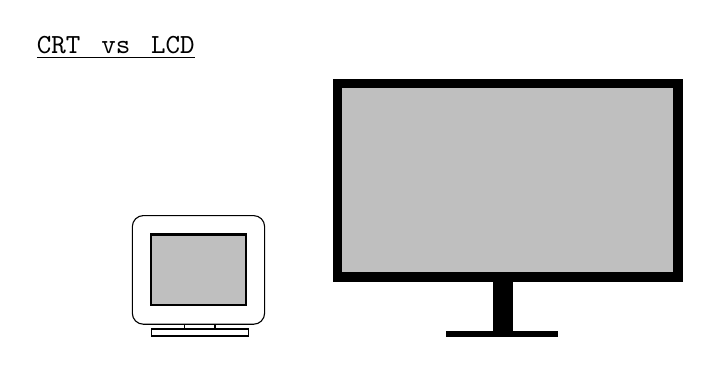
\begin{tikzpicture}[scale=0.3]


%Title
\node[above] at (2.5,15){$\mathtt{\Huge{\underline{CRT\ vs\ LCD}}}$}  ;


%Defining grey color
\colorlet{LighterMark}{black!25}

%CRT
\draw [thick,fill=LighterMark] (4,5) rectangle (8,8);
\draw [rounded corners] (3.2,4.2) rectangle (8.8,8.8);
\draw [] (5.4,4.2) rectangle (6.7,4);
\draw [] (4,4) rectangle (8.1,3.7);

%LCD
% cadre
\draw [ultra thick,fill=black] (11.8,6.1) rectangle (26.4,14.5);
%active screen
\draw [ultra thick,fill=LighterMark] (12,6.3) rectangle (26.2,14.3);
%bar
\draw [fill=black] (18.5,6.3)    rectangle (19.3,3.7);
%socle
\draw [fill=black] (16.5,3.7) rectangle (21.2,3.9);

\end{tikzpicture}
